\chead{Blatt 3}
\section*{Aufgabe 11}
Mittels Analyse der Buchstabenhäufigkeit ließ sich der Schlüssel für die
MASC-Chiffrierung (Hinweis!) als \verb/GOETHE/ bestimmen. Der entschlüsselte
Text lautet:
\begin{verbatim}
FRUEHDREIUHRSTAHLICHMICHAUSKARLSBADWEILMANMICHSONSTNICHTFORTGELASSENHAETTEDIEGES
ELLSCHAFTDIEDENACHTUNDZWANZIGSTENAUGUSTMEINENGEBURTSTAGAUFEINESEHRFREUNDLICHEWEI
SEFEIERNMOCHTEERWARBSICHWOHLDADURCHEINRECHTMICHFESTZUHALTENALLEINHIERWARNICHTLAE
NGERZUSAEUMENICHWARFMICHGANZALLEINNUREINENMANTELSACKUNDDACHSRANZENAUFPACKENDINEI
NEPOSTCHAISEUNDGELANGTEHALBACHTUHRNACHZWOTAANEINEMSCHOENENSTILLENNEBELMORGENDIEO
BERNWOLKENSTREIFIGUNDWOLLIGDIEUNTERNSCHWERMIRSCHIENENDASGUTEANZEICHENICHHOFFTENA
CHEINEMSOSCHLIMMENSOMMEREINENGUTENHERBSTZUGENIESSENUMZWOELFINEGERBEIHEISSEMSONNE
NSCHEINUNDNUNERINNERTEICHMICHDASSDIESERORTDIESELBEPOLHOEHEHABEWIEMEINEAATERSTADT
UNDICHFREUTEMICHWIEDEREINMALBEIKLAREMHIMMELUNTERDEMFUNFZIGSTENGRADEZUMITTAGZUESS
EN
\end{verbatim}
Dies ist der Anfang aus Goethes Reisebericht \flqq Italienischen Reise\frqq.

\section*{Aufgabe 12}
Wir bestimmen die kürzesten Gittervektoren mittels folgenden einfachen
Haskell-Programms:
\lstset{language=Haskell}
\begin{lstlisting}
-- kanonisches Skalarprodukt
(<*>) :: [Double] -> [Double] -> Double
(<*>) xs ys = sum $ zipWith (*) xs ys

---
-- Algorithmus zur Gauss-Reduktion
-- 'xs' ist der kuerzere Vektor!
gaussRed :: ([Double], [Double]) -> ([Double], [Double])
gaussRed (xs, ys) | lb < la = gaussRed (b, xs)  -- Schritt (3)
                  | otherwise = (xs, b)         -- Schritt (4)
        where   la = xs <*> xs
                -- Schritt (2)
                m = fromInteger $ round ( (xs <*> ys) / (xs <*> xs) ) 
                b = zipWith (-) ys (map (m*) xs) -- b := b - ma
                lb = b <*> b
\end{lstlisting}
Diese sind:
\begin{lstlisting}
> gaussRed ([10,31,51,-26],[-10,-40,-82,48])
	([-10,-13,11,-18],[10,22,20,-4])
\end{lstlisting}
woraus für die sukzessiven Minima folgt:
\[ \lambda_1(\Lambda) \approx 26.72, \lambda_2(\Lambda) \approx 31.62 \]
Die Gitterdeterminante ist
\[ \sqrt{\det\left(\begin{matrix}10728&-6770\\-6770&4338\end{matrix}\right)} = \sqrt{705164} \]

\section*{Aufgabe 13}
Die Gitterdeterminante ist
\[ \sqrt{\begin{vmatrix}1&t\\t&1\end{vmatrix}} = \sqrt{1-t^2} \]

\begin{table}[!ht]
	\subfloat[Gauß-Reduktion für $0 \leq t < \frac{1}{2}$]{
	\begin{tabular}{c|c|c|c|c}
		$a$&$b$&$\|a\|$&$\|b\|$&$\lfloor\mu\rceil$\\
		\hline
		$(1,0)$&$(t,\sqrt{1-t^2})$&$1$&$1$&$0$
	\end{tabular}
	}
	\subfloat[Gauß-Reduktion für $\frac{1}{2} < t < 1$]{
	\begin{tabular}{c|c|c|c|c}
		$a$&$b$&$\|a\|$&$\|b\|$&$\lfloor\mu\rceil$\\
		\hline
		$(1,0)$&$(t,\sqrt{1-t^2})$&$1$&$1$&$1$\\
		$(t-1,\sqrt{1-t^2})$&$(1,0)$&$\sqrt{2(1-t)}$&$1$&$0$
	\end{tabular}
	}
\end{table}

\noindent Die sukzessiven Minima für (a) sind $\lambda_1(\Lambda) = \lambda_2(\Lambda) =
1$, für (b) gilt $\lambda_1(\Lambda) = \sqrt{2(1-t)}, \ \lambda_2(\Lambda) = 1$.

Den Fall $t=\frac{1}{2}$ kann man einem der obigen Fälle zuordnen, je nach
Definiton der Rundungsoperation. Rundet man $\frac{1}{2}$ ab, so korrespondiert
dies mit dem Fall für $0 \leq t < \frac{1}{2}$. Wird aufgerundet, so hört man
nach dem ersten Schritt aus dem Fall für $\frac{1}{2} < t < 1$ auf, da die
Vektoren weiterhin gleiche Länge haben.

\section*{Aufgabe 14}
\begin{enumerate}[(1)]
	\item
		Nach Ausmultiplizieren der rechten Seite erhält man die Äquivalenzen
		\[ 0 \equiv x_1^2 + y_1^2 - 2(x_1x_2 + y_1y_2) \equiv x_2^2 + y_2^2 - 2(x_1x_2 + y_1y_2)\mod 7 \]
		Man stellt mittels folgenden Haskell-Programms fest, dass der
		gemischte Term $(x_1x_2 + y_1y_2) \equiv 0\mod 7$ ist:
		\begin{lstlisting}
> [ a | x1 <- [0..6], 
	x2 <- [0..6],
	y1 <- [0..6],
	y2 <- [0..6],
	let a = ( 2* (x1 * x2 + y1 * y2)) `mod` 7,
	(-a + x1^2 + y1^2) `mod` 7 == 0,
	(-a + x2^2 + y2^2) `mod` 7 == 0 ]
	
  [0]
		\end{lstlisting}
		Betrachtet man die Wertetabelle der Quadrate modulo 7

		\begin{tabular}{c|ccccccc}
			$n$&0&1&2&3&4&5&6\\
			\hline
			$n^2\mod 7$&0&1&4&2&2&4&1
		\end{tabular}

		so erkennt man, dass mit $a^2 + b^2 \equiv 0\mod7,\ a,b \in \Z$
		folgt, dass $a^2 \equiv b^2 \equiv 0\mod 7$ und damit auch $a
		\equiv b \equiv 0\mod7$. Somit gilt die Behauptung.
	\item
		Da die Gleichung
		$x_1^2+y_1^2=x_2^2+y_2^2=(x_1-x_2)^2+(y_1-y_2)^2$ gilt, ist
		nach (1) insbesondere auch $x_1^2+y_1^2\equiv x_2^2+y_2^2\equiv
		(x_1-x_2)^2+(y_1-y_2)^2\mod 7$ erfüllt und damit
		\[ x_1 \equiv x_2 \equiv y_1 \equiv y_2 \equiv 0\mod 7 \]
		d.h.
		\[ x_1 = k_1 \cdot 7,\quad x_2 = k_2 \cdot 7,\quad y_1 = k_3 \cdot 7,\quad y_2 = k_4 \cdot 7 \]
		Sei nun mindestens eines der $k_i$ ungleich $0$, dann muss
		dieses eine Potenz von $7$ sein, damit die Gleichung nach
		Reduktion modulo $7$ weiterhin erfüllt ist:
		\begin{eqnarray*}
			(7 k_1)^2+(7 k_3)^2&=&(7 k_2)^2+(7 k_4)^2=(7 k_1 - 7 k_2)^2 + (7 k_3 - 7 k_4)^2 \\
			\Leftrightarrow k_1^2+k_3^2&=&k_2^2+k_4^2=(k_1 - k_2)^2 + (k_3 - k_4)^2
		\end{eqnarray*}
		Führt man dies jedoch fort (Ausklammern von 7), so muss für die
		$k_i$, die nicht gleich $0$ sind, zuletzt eine $1$ stehen
		bleiben, was im Widerspruch zur Annahme steht, dass die
		Lösungen kongruent $0$ modulo $7$ sind.

		Somit sind alle $k_i$ gleich $0$ und damit auch $x_1, x_2, y_1$ und $y_2$.

	\item
		Die $6$ Gitterpunkte müssen auf einem Kreis liegen und aus
		$\Z^2$ sein. Da das Gitter in $\mathbb{R}^2$ liegt bilden zwei
		davon zusammen eine Gitterbasis. Die Basis mit $(-1)$
		multipliziert ergibt zwei weitere Gitterpunkte, die auf diesem
		Kreis liegen.

		\begin{center}
		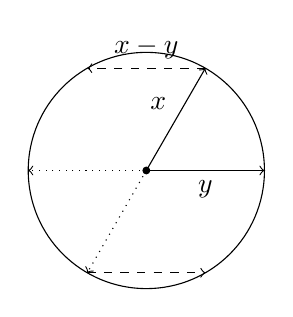
\begin{tikzpicture}
			\fill (0,0) circle (0.5mm);
			\draw (0,0) circle (1.5cm);
			\path (0,0) coordinate (origin);
			\path (60:1.5cm) coordinate (P);
			\path (120:1.5cm) coordinate (Q);
			\path (0:1.5cm) coordinate (R);
			\path (180:1.5cm) coordinate (S);
			\path (240:1.5cm) coordinate (T);
			\path (300:1.5cm) coordinate (U);
			\draw[->] (origin) -- node[anchor=south east] {$x$} (P);
			\draw[dashed,->] (P) -- node[anchor=south] {$x-y$} (Q);
			\draw[->] (origin) -- node[anchor=north] {$y$} (R);
			\draw[dotted,->] (origin) -- (S);
			\draw[dotted,->] (origin) -- (T);
			\draw[dashed,->] (T) -- (U);
		\end{tikzpicture}
		\end{center}

		Anhand dieser Skizze erkennt man, dass für die Längen der
		Gittervektoren $|x|^2 = |y|^2 = |x-y|^2$; dies ist genau die
		Gleichung aus (2). Da nur die triviale Lösung diese erfüllt
		existieren keine Gitter mit $6$ kürzesten Gittervektoren in
		$\Z^2$.
\end{enumerate}

\section*{Aufgabe 15}
Für $n \not\equiv 0\mod4$ ist die Matrix der Gitterbasis wie folgt aufgebaut:
\[
M_\Lambda = \begin{bmatrix} a_1 \\ a_2 \\ \vdots \\ a_n \end{bmatrix} = 
	\begin{bmatrix}
		2&2&0&\cdots&\cdots&0\\
		0&2&2&\ddots&&\vdots\\
		\vdots&\ddots&\ddots&\ddots&\ddots&\vdots\\
		\vdots&&\ddots&\ddots&\ddots&0\\
		\vdots&&&\ddots&2&2\\
		0&\cdots&\cdots&\cdots&0&4
	\end{bmatrix}
\]
Die Zeilensummen sind offensichtlich kongruent $0$ modulo $4$, die Einträge
kongruent modulo $2$. Damit erfüllen auch alle $\Z$-Linearkombiantionen diese
Bedingungen. In der anderen Richtung lässt sich jeder Vektor $(x_1,\dots,x_n)$
mit den genannten Eigenschaften als $\Z$-Linearkombination der gegebenen Matrix
darstellen wie folgt (dabei sind alle Einträge $x_i \equiv 0\mod2$, da
andernfalls die erste Bedingung verletzt wäre, denn eine Summe von $n
\not\equiv 0\mod4$ ungeraden Summanden ist nie durch $4$ teilbar):
\[ x = \frac{x_1}{2} a_1 + \frac{x_2-x_1}{2} a_2 + \cdots +
\frac{x_{n-1}-x_{n-2}+x_{n-3}-\cdots}{2} a_{n-1} +
\frac{x_n-x_{n-1}+x_{n-2}-\cdots}{4} a_n = (x_1, \dots x_n) \]
Dabei ist folgendes zu beachten:
\begin{eqnarray}
	\sum_{i=0}^{n-1} (-1)^i x_{n-i} &\equiv& k\mod 4 \\
	\sum_{i=0}^{n-1} x_{n-i} &\equiv& 0\mod 4 \text{ nach Voraussetzung} \\
	\nonumber (1) + (2): \sum_{i=0}^{\lfloor\frac{n}{2}\rfloor} 2 x_{n-2i} &\equiv& 0\mod 4
\end{eqnarray}
Da die $x_i$ gerade sind ist $k = 0$.

Die Gitterdeterminante berechnet sich analog zu Aufgabe 10, abgesehen vom
Faktor $2$ pro Zeile, d.h.
\[ \det(\Lambda_n) = \sqrt{4\cdot2^n} = 2^{\frac{n}{2} + 1},\ n \not\equiv 0\mod4 \]

Für $n \equiv 0\mod4$ wird in obiger Matrix $a_1$ durch den Einsvektor mit $n$
Einträgen ersetzt: 
\[
M_\Lambda = \begin{bmatrix} a_1 \\ a_2 \\ \vdots \\ a_n \end{bmatrix} = 
	\begin{bmatrix}
		1&1&1&\cdots&\cdots&1\\
		0&2&2&0&\cdots&0\\
		\vdots&\ddots&\ddots&\ddots&\ddots&\vdots\\
		\vdots&&\ddots&\ddots&\ddots&0\\
		\vdots&&&\ddots&2&2\\
		0&\cdots&\cdots&\cdots&0&4
	\end{bmatrix}
\]
Sind die $x_i$ gerade, so entspricht die Darstellung beliebiger $x$ mit den
geforderten Eigenschaften genau der obigen Argumentation. Bei ungeraden $x_i$
wird $a_1$ von dem Vektor $x$ abgezogen. Für den Rest gilt erneut obige
Argumentation, da nun alle $x_i$ gerade sind.

Für $n \geq 4, n$ Zweierpotenz ist diese Gitterbasis interessanterweise
äquivalent (nach Zeilen- und Spaltenumformungen) zu einem $\log_2(n)$-fachen
Tensorprodukt der \textsc{Hadamard}-Matrix (ohne den Skalierungsfaktor
$\frac{1}{\sqrt{2}}$):
\[ M_\Lambda = (\sqrt{2}H)^{\otimes\log_2(n)} = \begin{bmatrix} 1&1\\1&-1
\end{bmatrix}^{\otimes\log_2(n)} \]
Da die \textsc{Hadamard}-Matrizen unitär sind sind deren Determinanten gleich
$1$. Da wir aus jeder Zeile den Faktor $\sqrt{2}^{\log_2(n)}$ herausziehen
ergibt sich für die Determinante von $M_\Lambda \cdot M_\Lambda^T$ in diesen
Fällen $\sqrt{\det(M_\Lambda \cdot M_\Lambda^T)} = n^{\frac{n}{4}} =
\det{\Lambda_n},\ n \equiv 0\mod4, n \text{ Zweierpotenz}$
